% !TeX root = ../../presentation-local.tex

\section{Coq Programming}

\begin{frame}{Coq}
\begin{itemize}
  \item Coq is an interactive theorem prover
  \item Main idea: Propositions as Types, Proofs as Terms (Curry-Howard-Correspondence)
  \item One can define
    \begin{itemize}
      \item Inductive \textbf{Types (Propositions)}
      \item Well-typed \textbf{Terms (Proofs)}
    \end{itemize}
  \item The underlying language Gallina
    \begin{itemize}
      \item is a dependently-typed functional programming language
      \item implements the Calculus of Inductive Constructions
      \item is not Turing-complete (every term has a normal form)
    \end{itemize}
\end{itemize}
\begin{center}
  
\includegraphics[width=0.33\textwidth]{content/theorem-proving/images/coq.png}
\end{center}
\end{frame}

\begin{frame}{Getting started with Coq}
\begin{enumerate}
  \item Installation
    \begin{itemize}
      \item Win/Mac: Download from \url{https://coq.inria.fr/}
      \item Linux: We recommend installation via OPAM \url{https://coq.inria.fr/opam/www/using.html}
    \end{itemize}
  \item IDE
    \begin{itemize}
      \item Recommendation: Coq IDE, shipped with Coq (see screenshot)
      \item Popular plugin for Emacs: Proof General
    \end{itemize}
\end{enumerate}
\begin{center}
  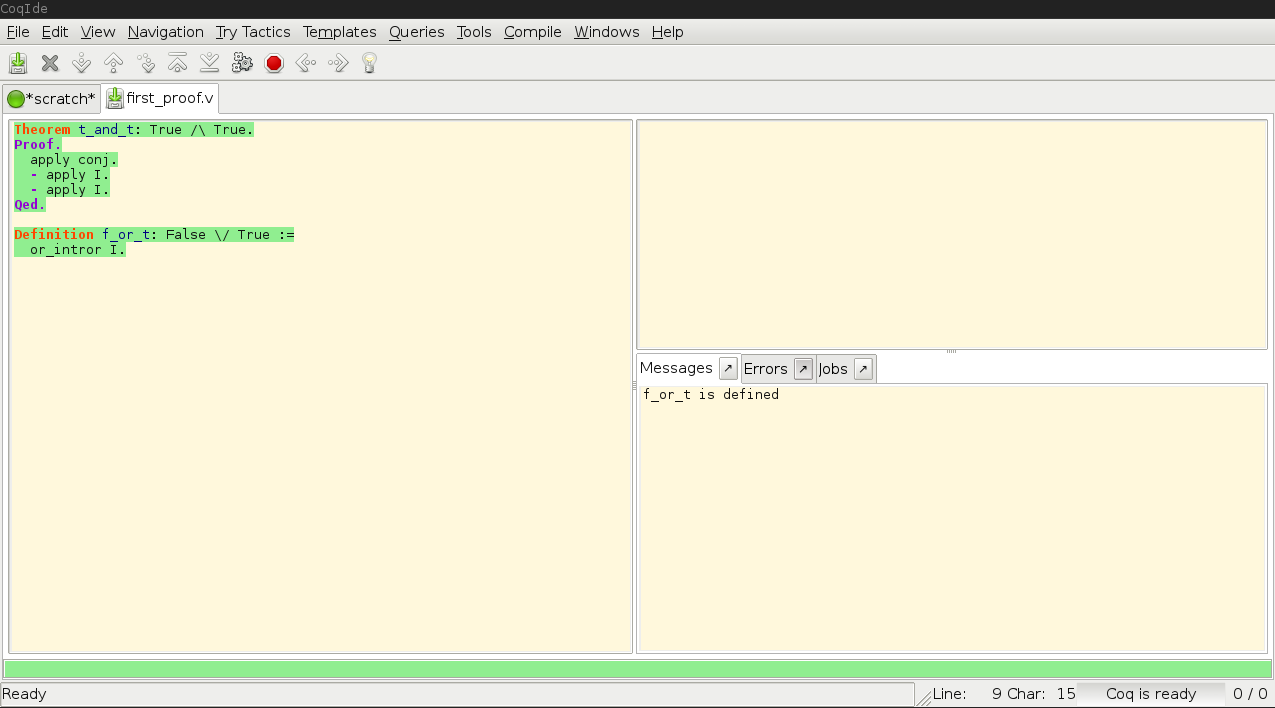
\includegraphics[width=0.8\textwidth]{content/theorem-proving/images/coqide.png}
\end{center}
\end{frame}

\begin{frame}[fragile]{Coq Programming\small~~ (Inductive Data Types)}
\begin{itemize}
  \item An inductive data type definition introduces a \textbf{new type} and \textbf{new well-typed terms}
\lstinputlisting{content/theorem-proving/coq/snippets/bool_nat.v}

\pause

\item \lstinline|bool|, \lstinline|nat| are types
\item \lstinline|true|, \lstinline|false|, \lstinline|O|, \lstinline|S| are value constructors
\end{itemize}
\end{frame}

\begin{frame}[fragile]{Coq Programming\small~~ (Definitions)}
\begin{itemize}
  \item A \lstinline|Definition| gives a name to a term
  \lstinputlisting{content/theorem-proving/coq/snippets/three.v}

  \pause

  \item Definitions can be unfolded, which is a kind of \textit{reduction}

  \item Two terms are \textit{convertible} ($\equiv$) if they reduce to the same term

  \item The terms \lstinline|S two| and \lstinline|three| are convertible
\begin{lstlisting}
  S two
=== S(S(S O))
=== three
\end{lstlisting}

  \pause

  \item \textit{Intuition:} Convertibility is \say{syntactic equality up-to certain manipulations}
\end{itemize}
\end{frame}

\begin{frame}[fragile]{Coq Programming\small~~ (Functions, Pattern Matching)}
\begin{itemize}
  \item We can define functions that use pattern matching
  \lstinputlisting{content/theorem-proving/coq/snippets/negb.v}

  \pause

  \item \lstinline|fun x => ...| introduces a function
  \item \lstinline!match ... with | ... end! pattern-matches

  \pause

  \item Both constructs introduce a form of reduction and thus of convertibility
\begin{lstlisting}
  negb true
=== (fun x => ...) true
=== match true with | true => false | ...
=== false
\end{lstlisting}
\end{itemize}
\end{frame}

\begin{frame}[fragile]{Coq Programming\small~~ (Short Notation for Functions)}
\begin{itemize}
  \item Recall our function
  \lstinputlisting{content/theorem-proving/coq/snippets/negb.v}
  \item We can use the following short notation
  \lstinputlisting{content/theorem-proving/coq/snippets/negb_param.v}
\end{itemize}
\end{frame}

\begin{frame}[fragile]{Coq Programming\small~~ (Type-Checking)}
\begin{itemize}
  \item In Coq, every term must be well-typed
  \item What does that mean?
  \begin{itemize}
    \item We write $Γ ⊢ t: T$ and call it a \textit{(typing) judgement}
    \item \say{Under context $Γ$, term $t$ has type $T$}
    \item Context $Γ$ is a list of items $t: T$
    \item ~\\[-3em]
    \begin{alignat*}{2}
      \text{E.g., we have} &\quad x: \mathit{bool} ~&⊢ \mathit{negb}~x: \mathit{bool}\\
      \text{...but \textbf{not}} &\quad x: \mathit{nat} ~&⊢ \mathit{negb}~x: \mathit{bool}
    \end{alignat*}
  \end{itemize}

  \pause

  \item Coq can \textit{try to find} a type $T$ for $Γ, t$ (a.k.a. \textbf{type inference}, generally undecidable)

  \pause

  \item Coq \textit{decides} for a given judgement whether it holds (a.k.a. \textbf{type-checking})
\end{itemize}
\end{frame}

\begin{frame}[fragile]{Coq Programming\small~~ (Type-Checking, Reducing in Coq)}
\begin{itemize}
  \item Type-infer terms and compute (reduce) terms
\begin{lstlisting}[mathescape=true]
Check (negb true).   $\leadsto$  negb true: bool
Compute (negb true). $\leadsto$  false: bool
\end{lstlisting}
  \begin{itemize}
    \item Here, the context $Γ$ is considered by Coq but not explicitly output
  \end{itemize}
\end{itemize}
\end{frame}

\begin{frame}[fragile]{Coq Programming\small~~ (Recursive Functions)}
\begin{itemize}
  \item We can define recursive functions
  \lstinputlisting{content/theorem-proving/coq/snippets/plus_param.v}

  \pause

  \item Above was really a short notation for the following:
  \lstinputlisting{content/theorem-proving/coq/snippets/plus.v}
\end{itemize}
\end{frame}

\begin{frame}[fragile]{Coq Programming\small~~ (Recursion must be structural)}
\lstinputlisting{content/theorem-proving/coq/snippets/plus_param.v}
\begin{itemize}
  \item Recursive functions in Coq \textbf{always terminate} because only \textit{structural recursion} is allowed

  \pause

  \item Structural recursion means that recursion is only applied to sub-structures
  \item Here: \lstinline|m'| is a sub-structure of \lstinline|S m'|

  \pause

  \item Why this restriction? Remember: Proofs are programs, and non-terminating proofs must be avoided!\\
  (more later)
\end{itemize}
\end{frame}

\begin{frame}{Coq Programming\small~~ (Prelude and Notation)}
\begin{itemize}
  \item Standard data types, functions, notation are pre-defined via the Prelude\footnote{\scriptsize\url{https://coq.inria.fr/library/Coq.Init.Prelude.html}}
  \item This allows us to write a term like \lstinline|3 + 2| instead of \lstinline|plus S(S(S O)) S(S O)|.
  \item We use the nice notation from now on wherever possible
\end{itemize}
\end{frame}

\begin{frame}[fragile]{Coq Programming\small~~ (Polymorphic Data Types, 1)}
\begin{itemize}
  \item It is often useful to parameterize a data type to avoid multiple definitions such as \lstinline|natList|, \lstinline|boolList| etc.
\lstinputlisting{content/theorem-proving/coq/snippets/list_param.v}

  \pause

  \item We say that \lstinline|list| is \textit{polymorphic} in its \textit{parameter} \lstinline|X|

  \pause

  \item We say that \lstinline|list| is a \textit{type constructor} (a function that constructs a type)

  \pause

  \item Applying this type constructor yields

  \begin{itemize}
    \item \lstinline|list nat:  |\lstinline| Type|
    \item \lstinline|list bool: |\lstinline|Type|
    \item ...
  \end{itemize}
\end{itemize}
\end{frame}

\begin{frame}[fragile]{Coq Programming\small~~ (Polymorphic Data Types, 2)}
In the parameterized definition
\lstinputlisting{content/theorem-proving/coq/snippets/list_param.v}
... the parameter \lstinline|X| can be \say{multiplied-out} to ...
\lstinputlisting{content/theorem-proving/coq/snippets/list.v}
\begin{itemize}
  \pause

  \item The following judgements are introduced
  \begin{itemize}
    \item \lstinline|list: Type -> Type|
    \item \lstinline|nil:| ~\lstinline| forall(X: Type), list X|
    \item \lstinline|cons: forall(X: Type), X -> list X -> list X|
  \end{itemize}

  \pause

  \item The definitions are isomorphic (modulo technicalities), but the parameterized definition emphasises that \textit{the structure} of \lstinline|list| terms is independ. of the choice of \lstinline|X|
\end{itemize}
\end{frame}

\begin{frame}[fragile]{Coq Programming\small~~ (Implicit Parameters, 1)}
\lstinputlisting{content/theorem-proving/coq/snippets/list_param.v}
\begin{itemize}
  \item Recall that this introduces the judgements\\
  \lstinline|nil:| ~~\,\lstinline|forall(X: Type), list X|\\
  \lstinline|cons: forall(X: Type), X -> list X -> list X|

  \pause

  \item ... so the value constructors must be instantiated, e.g.\\
  \lstinline|cons nat 42 (nil nat): list nat|

  \pause

  \item 42 is a \lstinline|nat|, so \lstinline|X| \textit{must} be instantiated by \lstinline|nat|. Can we let Coq infer this and simply write\\
  \lstinline|cons 42 nil: list nat|\\
  instead?

  \pause

  \item Yes! (See next slide)
\end{itemize}
\end{frame}

\begin{frame}[fragile]{Coq Programming\small~~ (Implicit Parameters, 2)}

\begin{itemize}
  \item Recall our example term:\\
  \lstinline|cons nat 42 (nil nat) : list nat|

  \pause

  \item We can manually mark arguments as implicit or enable this by default via
  \lstinputlisting{content/theorem-proving/coq/snippets/list_param_implicit.v}

  \pause

  \item \lstinline|X| is strictly implicit for \lstinline|cons| (alway inferrable)

  \pause

  \item \lstinline|X| is contextually implicit for \lstinline|nil| (sometimes inferrable)

  \pause

  \item This allows to write the example term as:\\
  \lstinline|cons 42 nil : list nat|

  \pause

  \item But we lack the context to infer
  \lstinline|nil : list nat|

  \pause

  \item There is further notation\footnote{use \lstinline|Require Import Coq.Lists.List.|}: \lstinline|42::nil : list nat|
\end{itemize}
\end{frame}
